\documentclass[12pt]{article}

\usepackage{geometry}
\geometry{margin = 1in,top =0.12\paperheight, headheight=\paperheight}
\usepackage[export]{adjustbox}
\usepackage{array}
\usepackage{amsmath}
\usepackage{amsfonts}
\usepackage{fancyhdr}
\usepackage{lastpage}
\usepackage{xcolor}
\usepackage{comment}
\pagestyle{fancy}
\fancyhf{}
\rhead{Written Assignment, Page \thepage}
\lhead{MATH211}
\chead{
\includegraphics[width = 0.15\textwidth]{MCLogo-Bck.png}}


%\renewcommand{\footrulewidth}{0.4pt}

\usepackage{enumitem}
\usepackage{pifont}
\usepackage{graphicx}
\graphicspath{{../img}}

\newtheorem{theorem}{Theorem}
\newtheorem{exercise}{Exercise}


\newcommand{\R}{\mathbb R}
\newcommand{\e}{{\rm e}}
\newcommand{\inpr}[1]{\left\langle#1\right\rangle}
\newcommand{\norm}[1]{\lVert #1 \rVert}
\newcommand{\abs}[1]{\lvert #1 \rvert}
\newcommand{\vv}{\mathbf v}
\newcommand{\uv}{\mathbf u}

\DeclareMathOperator{\xd}{d\!}
\DeclareMathOperator{\proj}{proj}

\title{}
\date{}

\begin{document}
\noindent
{\bf Problem.}
Using vectors, prove the Law of Sines: if $\mathbf a$, $\mathbf b$, and $\mathbf c$ are the three sides of the triangle shown in the figure, then
\[
\frac{\sin A}{\norm{\mathbf a}}=\frac{\sin B}{\norm{\mathbf b}}=\frac{\sin C}{\norm{\mathbf c}}.
\]
({\it Hint:} Use the relation between cross products and triangle areas.)
\begin{figure}[h]
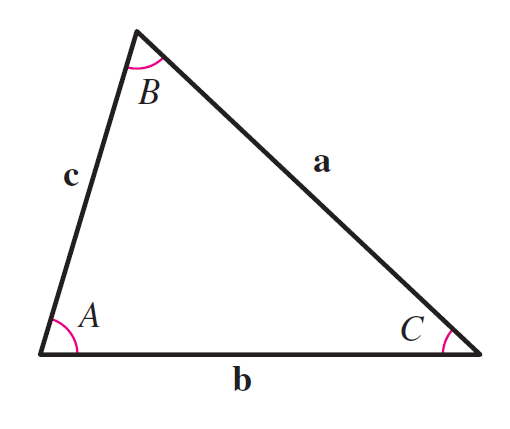
\includegraphics[width=0.3\textwidth, right]{sinelaw.png}
\end{figure}

\end{document}